% Options for packages loaded elsewhere
\PassOptionsToPackage{unicode}{hyperref}
\PassOptionsToPackage{hyphens}{url}
%
\documentclass[
]{article}
\usepackage{amsmath,amssymb}
\usepackage{lmodern}
\usepackage{ifxetex,ifluatex}
\ifnum 0\ifxetex 1\fi\ifluatex 1\fi=0 % if pdftex
  \usepackage[T1]{fontenc}
  \usepackage[utf8]{inputenc}
  \usepackage{textcomp} % provide euro and other symbols
\else % if luatex or xetex
  \usepackage{unicode-math}
  \defaultfontfeatures{Scale=MatchLowercase}
  \defaultfontfeatures[\rmfamily]{Ligatures=TeX,Scale=1}
\fi
% Use upquote if available, for straight quotes in verbatim environments
\IfFileExists{upquote.sty}{\usepackage{upquote}}{}
\IfFileExists{microtype.sty}{% use microtype if available
  \usepackage[]{microtype}
  \UseMicrotypeSet[protrusion]{basicmath} % disable protrusion for tt fonts
}{}
\makeatletter
\@ifundefined{KOMAClassName}{% if non-KOMA class
  \IfFileExists{parskip.sty}{%
    \usepackage{parskip}
  }{% else
    \setlength{\parindent}{0pt}
    \setlength{\parskip}{6pt plus 2pt minus 1pt}}
}{% if KOMA class
  \KOMAoptions{parskip=half}}
\makeatother
\usepackage{xcolor}
\IfFileExists{xurl.sty}{\usepackage{xurl}}{} % add URL line breaks if available
\IfFileExists{bookmark.sty}{\usepackage{bookmark}}{\usepackage{hyperref}}
\hypersetup{
  pdftitle={Project},
  pdfauthor={Chris Martin},
  hidelinks,
  pdfcreator={LaTeX via pandoc}}
\urlstyle{same} % disable monospaced font for URLs
\usepackage[margin=1in]{geometry}
\usepackage{color}
\usepackage{fancyvrb}
\newcommand{\VerbBar}{|}
\newcommand{\VERB}{\Verb[commandchars=\\\{\}]}
\DefineVerbatimEnvironment{Highlighting}{Verbatim}{commandchars=\\\{\}}
% Add ',fontsize=\small' for more characters per line
\usepackage{framed}
\definecolor{shadecolor}{RGB}{248,248,248}
\newenvironment{Shaded}{\begin{snugshade}}{\end{snugshade}}
\newcommand{\AlertTok}[1]{\textcolor[rgb]{0.94,0.16,0.16}{#1}}
\newcommand{\AnnotationTok}[1]{\textcolor[rgb]{0.56,0.35,0.01}{\textbf{\textit{#1}}}}
\newcommand{\AttributeTok}[1]{\textcolor[rgb]{0.77,0.63,0.00}{#1}}
\newcommand{\BaseNTok}[1]{\textcolor[rgb]{0.00,0.00,0.81}{#1}}
\newcommand{\BuiltInTok}[1]{#1}
\newcommand{\CharTok}[1]{\textcolor[rgb]{0.31,0.60,0.02}{#1}}
\newcommand{\CommentTok}[1]{\textcolor[rgb]{0.56,0.35,0.01}{\textit{#1}}}
\newcommand{\CommentVarTok}[1]{\textcolor[rgb]{0.56,0.35,0.01}{\textbf{\textit{#1}}}}
\newcommand{\ConstantTok}[1]{\textcolor[rgb]{0.00,0.00,0.00}{#1}}
\newcommand{\ControlFlowTok}[1]{\textcolor[rgb]{0.13,0.29,0.53}{\textbf{#1}}}
\newcommand{\DataTypeTok}[1]{\textcolor[rgb]{0.13,0.29,0.53}{#1}}
\newcommand{\DecValTok}[1]{\textcolor[rgb]{0.00,0.00,0.81}{#1}}
\newcommand{\DocumentationTok}[1]{\textcolor[rgb]{0.56,0.35,0.01}{\textbf{\textit{#1}}}}
\newcommand{\ErrorTok}[1]{\textcolor[rgb]{0.64,0.00,0.00}{\textbf{#1}}}
\newcommand{\ExtensionTok}[1]{#1}
\newcommand{\FloatTok}[1]{\textcolor[rgb]{0.00,0.00,0.81}{#1}}
\newcommand{\FunctionTok}[1]{\textcolor[rgb]{0.00,0.00,0.00}{#1}}
\newcommand{\ImportTok}[1]{#1}
\newcommand{\InformationTok}[1]{\textcolor[rgb]{0.56,0.35,0.01}{\textbf{\textit{#1}}}}
\newcommand{\KeywordTok}[1]{\textcolor[rgb]{0.13,0.29,0.53}{\textbf{#1}}}
\newcommand{\NormalTok}[1]{#1}
\newcommand{\OperatorTok}[1]{\textcolor[rgb]{0.81,0.36,0.00}{\textbf{#1}}}
\newcommand{\OtherTok}[1]{\textcolor[rgb]{0.56,0.35,0.01}{#1}}
\newcommand{\PreprocessorTok}[1]{\textcolor[rgb]{0.56,0.35,0.01}{\textit{#1}}}
\newcommand{\RegionMarkerTok}[1]{#1}
\newcommand{\SpecialCharTok}[1]{\textcolor[rgb]{0.00,0.00,0.00}{#1}}
\newcommand{\SpecialStringTok}[1]{\textcolor[rgb]{0.31,0.60,0.02}{#1}}
\newcommand{\StringTok}[1]{\textcolor[rgb]{0.31,0.60,0.02}{#1}}
\newcommand{\VariableTok}[1]{\textcolor[rgb]{0.00,0.00,0.00}{#1}}
\newcommand{\VerbatimStringTok}[1]{\textcolor[rgb]{0.31,0.60,0.02}{#1}}
\newcommand{\WarningTok}[1]{\textcolor[rgb]{0.56,0.35,0.01}{\textbf{\textit{#1}}}}
\usepackage{graphicx}
\makeatletter
\def\maxwidth{\ifdim\Gin@nat@width>\linewidth\linewidth\else\Gin@nat@width\fi}
\def\maxheight{\ifdim\Gin@nat@height>\textheight\textheight\else\Gin@nat@height\fi}
\makeatother
% Scale images if necessary, so that they will not overflow the page
% margins by default, and it is still possible to overwrite the defaults
% using explicit options in \includegraphics[width, height, ...]{}
\setkeys{Gin}{width=\maxwidth,height=\maxheight,keepaspectratio}
% Set default figure placement to htbp
\makeatletter
\def\fps@figure{htbp}
\makeatother
\setlength{\emergencystretch}{3em} % prevent overfull lines
\providecommand{\tightlist}{%
  \setlength{\itemsep}{0pt}\setlength{\parskip}{0pt}}
\setcounter{secnumdepth}{-\maxdimen} % remove section numbering
\ifluatex
  \usepackage{selnolig}  % disable illegal ligatures
\fi

\title{Project}
\author{Chris Martin}
\date{08/12/2021}

\begin{document}
\maketitle

\hypertarget{abstract}{%
\subsection{Abstract}\label{abstract}}

\hypertarget{introduction}{%
\subsection{Introduction}\label{introduction}}

The purpose of this report is to detail to extensions made to the dsims
R package and conduct analysis to compare the abundance estimates
generated through a design based approach, distance sampling, and a
model based approach, density surface modelling. This will allow
researchers the opportunity to use the best possible model to fit the
circumstances of their own study.

\hypertarget{background-research}{%
\subsection{Background research}\label{background-research}}

Distance sampling is an approach to estimating population abundance and
density by surveying a small portion

need to define truncation distance, detection function, abundance and
density from literature.

explanation of how the ds and dsm models generate their abundance
estimates in R and under what circumstances one may be better than the
other to inform potential comparisons

\hypertarget{distance-sampling-simulations}{%
\subsection{Distance Sampling
Simulations}\label{distance-sampling-simulations}}

All the material in this section is based on Buckland et al (2015) Prior
to the simulation for a particular design being run, a number of objects
must be first be defined. The first object is the study region, this can
either be the default generated by R or user defined from a shapefile.
Following this, a spatial distribution or density surface must be
defined, from which animal locations can be generated based on the
population description. The desired population size can be user defined
and set for a series of simulations or be generated based on the spatial
distribution supplied by the user. The desired truncation distance must
then be defined and based on this an appropriate design can be
generated. The main considerations when constructing the design are the
type, either line or point transects and the desired number or length of
transects. If line transects are used, the design angle may be altered
from its default of 0. Based on the design, a set of survey transects
can be generated, during which the detection process is simulated. The
user can then define a detection function, based on either a half normal
(`hn'), hazard rate (`hr') or uniform distribution (`uf') with a defined
scale parameter and the desired truncation distance \emph{w}. Therefore
for an animal at distance \emph{x} from the closest transect the
probability of the animal being detected is given by the detection
function eveluated at \emph{x}, provided \emph{x} \le \emph{w}.

\hypertarget{modelling}{%
\subsection{Modelling}\label{modelling}}

the simulation was initially tested using the default region generated
by dsims with a point transect design aiming for 25 points with a
truncation distance of 60. A test density was then constructed for the
region with high and low spots as seen below with relatively gently
gradients.

\begin{Shaded}
\begin{Highlighting}[]
\CommentTok{\#plot(density, region) }
\end{Highlighting}
\end{Shaded}

A population description was then constructed based on this density
surface with a population of 1000 to start. A detection function was
then defined as a half normal with scale parameter of 30. This produces
the following detection function: \texttt{\{r\}\ plot(detect,\ pop.des)}

A prediction grid is then constructed across the study region and is the
same for each run of the simulation.

The simulation loop then begins. For each iteration, a new survey
constructed. From this, the observation data and segmented data is
extracted. Based on this data, both a distance sampling model and
density surface model are constructed, with the degrees of freedom in
the dsm model being restricted to the number of point transects and its
family being tweedie. the abundance estimates are extracted from both
models and stored.

\hypertarget{results}{%
\subsection{results}\label{results}}

Having completed 2000 bootstrap simulations for both the distance
sampling and density surface models, we can now examine and compare
these to give us an insight into the circumstances under which a
particular model is better of worse than the other. For the initial
default region, the histograms of both the distance sampling and dsm
abundance estimates are displayed below:

\begin{Shaded}
\begin{Highlighting}[]
\NormalTok{default.dsm }\OtherTok{\textless{}{-}} \FunctionTok{read.csv}\NormalTok{(}\StringTok{\textquotesingle{}dsm.estimates.region.csv\textquotesingle{}}\NormalTok{)}
\NormalTok{default.ds }\OtherTok{\textless{}{-}} \FunctionTok{read.csv}\NormalTok{(}\StringTok{\textquotesingle{}ds.estimates.region.csv\textquotesingle{}}\NormalTok{)}

\FunctionTok{hist}\NormalTok{(default.dsm}\SpecialCharTok{$}\NormalTok{x, }\AttributeTok{main =} \StringTok{\textquotesingle{}Histogram of DSM estimates\textquotesingle{}}\NormalTok{)}
\end{Highlighting}
\end{Shaded}

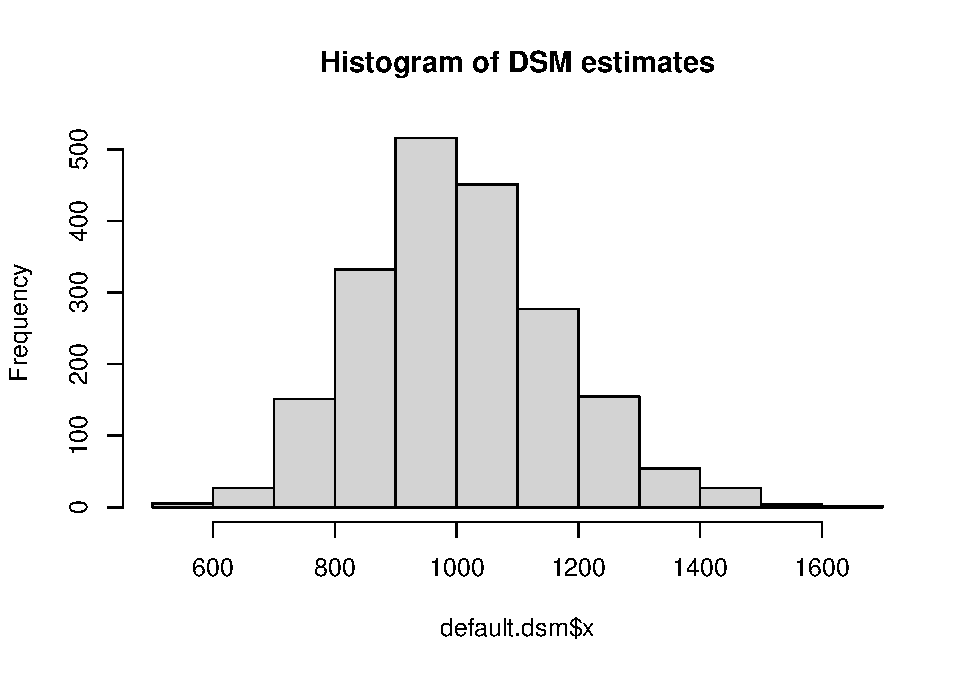
\includegraphics{project-report_files/figure-latex/unnamed-chunk-2-1.pdf}

\begin{Shaded}
\begin{Highlighting}[]
\FunctionTok{hist}\NormalTok{(default.ds}\SpecialCharTok{$}\NormalTok{x, }\AttributeTok{main =} \StringTok{\textquotesingle{}Histogram of DS estimates\textquotesingle{}}\NormalTok{)}
\end{Highlighting}
\end{Shaded}

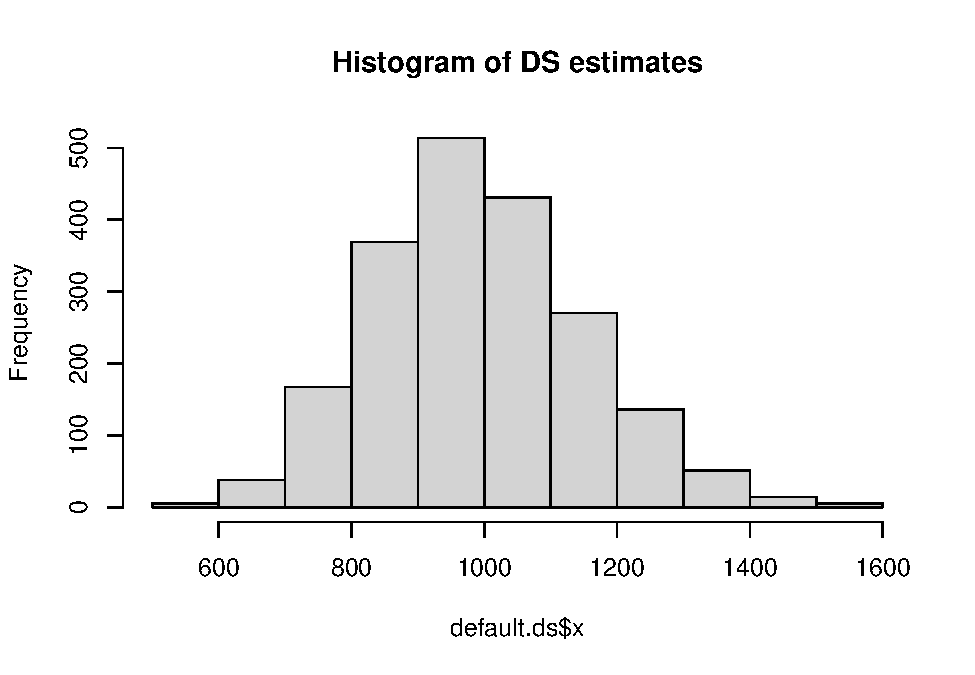
\includegraphics{project-report_files/figure-latex/unnamed-chunk-2-2.pdf}

These plots show somewhat similar data as we would expect since both
estimates are generated by the same data set. If we now compare the
means and 95\% confidence intervals:

\begin{Shaded}
\begin{Highlighting}[]
\FunctionTok{mean}\NormalTok{(default.dsm}\SpecialCharTok{$}\NormalTok{x)}
\end{Highlighting}
\end{Shaded}

\begin{verbatim}
## [1] 1007.034
\end{verbatim}

\begin{Shaded}
\begin{Highlighting}[]
\FunctionTok{mean}\NormalTok{(default.ds}\SpecialCharTok{$}\NormalTok{x)}
\end{Highlighting}
\end{Shaded}

\begin{verbatim}
## [1] 992.7283
\end{verbatim}

\begin{Shaded}
\begin{Highlighting}[]
\FunctionTok{quantile}\NormalTok{(default.dsm}\SpecialCharTok{$}\NormalTok{x, }\FunctionTok{c}\NormalTok{(}\FloatTok{0.025}\NormalTok{, }\FloatTok{0.975}\NormalTok{))}
\end{Highlighting}
\end{Shaded}

\begin{verbatim}
##      2.5%     97.5% 
##  722.5187 1348.1308
\end{verbatim}

\begin{Shaded}
\begin{Highlighting}[]
\FunctionTok{quantile}\NormalTok{(default.ds}\SpecialCharTok{$}\NormalTok{x,}\FunctionTok{c}\NormalTok{(}\FloatTok{0.025}\NormalTok{, }\FloatTok{0.975}\NormalTok{))}
\end{Highlighting}
\end{Shaded}

\begin{verbatim}
##      2.5%     97.5% 
##  713.5775 1328.6599
\end{verbatim}

It can be seen that the dsm method appears to xxx the true population
while the distance sampling method does xxx. Examining the confidence
intervals for both methods, the interval for the dsm model is in this
case wider than that of the ds model, indicating it is slightly less
accurate in the case of this region and density surface.

\hypertarget{conclusion}{%
\subsection{conclusion}\label{conclusion}}

\end{document}
